%%%%%%%%%%%%%%%%%%%%%%
% Signal selection   %
%%%%%%%%%%%%%%%%%%%%%%


\begin{sidewaystable}[p]
\centering
\caption{Cutflow table, event counts are normalized to $19.7\fbinv$. The signal is the
$m_{\tilde{g}}=1000\GeV$, $m_{\stopone}=325\GeV$, $m_{\lsp}=300\GeV$ point of the
T1ttcc scan. The row corresponding to ``$n_{PV} > 0$'' gives the event counts after applying the
cleaning filters, pileup reweighting, top \pt reweighting for $t\bar{t}$, ISR reweighting for
signal, and the requirement of at least one good primary vertex. The column indicating the total
number of events also includes some smaller processes that only contribute at the early stages of
the event selection. 
The cross sections used for each sample are listed in the second row.}
\vspace{1ex}
{\scriptsize
\begin{tabular}{ l | c  c  c  c  c  c  c  c  c | c  c  c }
%\begin{tabular}{ l || c  c  c  c  c  c  c  c  c | c || c || c }
%\begin{tabular}{| l || c | c | c | c | c | c | c | c | c | c || c || c || c |}
\toprule
Selection & Multijet & $t\bar{t}$ & $\W{\rightarrow}\ell\nu+$jets & Diboson & Single top &
$\cPZ{\rightarrow}\nu\nu+$jets & DY${\rightarrow}\ell\ell+$jets & Triboson & $t\bar{t}V$ & Total &
Signal & Data\\ 
 & $10.4\times 10^7$ pb & 245.8 pb & 111.5 pb & 95.4 pb & 114.9 pb & 588.3 pb & 22.6 pb & 0.69 pb &
1.88 pb & & 0.02435 pb & \\ 
 \midrule
% & 10.4e+07 pb & 245.8 pb & 111.5 pb & 95.4 pb & 114.9 pb & 588.3 pb & 22.6 pb & 0.69 pb & 1.88 pb & 121 pb & & 0.0243547 pb & \\ \hline \hline
No selection & $2.1\times 10^{11}$ & $4.9\times 10^6$ & $2.2\times 10^6$ & $1.9\times 10^6$ & $2.3\times 10^6$ & $1.2\times 10^7$ & $4.5\times 10^5$ & $1.2\times 10^4$ & $3\times 10^4$ & $2.1\times 10^{11}$ & 499 &  \\
$n_{PV} > 0$ & $1.05\times 10^{11}$ & $4.42\times 10^6$ & $2.02\times 10^6$ & $1.08\times 10^6$ & $1.72\times 10^6$ & $2.87\times 10^6$ & $3.7\times 10^5$ & $8.46\times 10^3$ & $2.6\times 10^4$ & $1.05\times 10^{11}$ & 479 & \\
$n_j \geq 3$ & $2.04\times 10^{10}$ & $4.08\times 10^6$ & $1.51\times 10^6$ & $5.19\times 10^5$ & $1.10\times 10^6$ & $6.24\times 10^5$ & $3.06\times 10^5$ & $5.64\times 10^3$ & $2.49\times 10^4$ & $2.05\times 10^{10}$ & 472 &  \\
$\pt(j_1) > 200\GeV$ & $1.82\times 10^8$ & $2.88\times 10^5$ & $4.36\times 10^5$ & $1.86\times 10^4$ & $6.08\times 10^4$ & $5.89\times 10^4$ & $6.61\times 10^4$ & 924 & $5.24\times 10^3$  & $1.82\times 10^8$ & 403 & \\
$M_R \,{>}\, 800, R^2 \,{>}\, 0.08$ & $3.47\times 10^4$ & $5.83\times 10^3$ & $1.17\times 10^4$ & 309 & 900 & $3.25\times 10^3$ & 422 & 40.2 & 183 & 57557 & 224 & \\
Trigger & $3.15\times 10^4$ & $5.12\times 10^3$ & $9.38\times 10^3$ & 249 & 786 & $2.32\times 10^3$ & 367 & 36.4 & 166 & 50164 & 216 & 67037 \\
\midrule
no lepton & $3.09\times 10^4$ & $1.87\times 10^3$ & $3.75\times 10^3$ & 96.3 & 311 & $2.30\times 10^3$ & 145 & 12.6 & 58.5 & 39666 & 142 & 56220 \\
\midrule[.02em]
$n_b \geq 1$ & $9.37\times 10^3$ & $1.51\times 10^3$ & 590 & 25.2 & 226 & 302 & 29.0 & 4.48 & 46.3 & 12187 & 119 & 18164 \\
$n_W \geq 1$ & 841 & 332 & 56.4 & 8.52 & 56.7 & 22.1 & 5.28 & 1.98 & 9.68 & 1350 & 28 & 1817  \\
S & 14.8 & 90.4 & 23.1 & 3.7 & 11.7 & 12.7 & 0.59 & 0.98 & 2.6 & 160 & 23.4 & 187 \\
\midrule[.02em]
$n_b = 0$ & $1.25\times 10^4$ & 98.3 & $1.70\times 10^3$ & 35.6 & 25.9 & $1.25\times 10^3$ & 46.5 & 4.19 & 3.56 & 15691 & 5.65 & 20667 \\
$n_{aW} \geq 1$ & 1519 & 18.7 & 204 & 8.36 & 7.40 & 158 & 5.41 & 0.751 & 0.819 & 1923 & 0.667 & 2712 \\
Q & 1447 & 10.6 & 93.1 & 3.88 & 3.94 & 38.9 & 3.68 & 0.28 & 0.52 & 1603 & 0.07 & 2240 \\
\midrule
1 lepton & 585.9 & $2.74\times 10^3$ & $5.52\times 10^3$ & 132 & 421 & 22.1 & 164 & 19.2 & 88.5 & 9699 & 65.0 & 10008 \\
\midrule[.02em]
$n_b \geq 1$ & 236.7 & $2.17\times 10^3$ & 625 & 29.9 & 301 & 4.14 & 28.7 & 5.36 & 68.3 & 3470 & 54 & 3930 \\
$n_W \geq 1$ & 24.3 & 496 & 61.6 & 10.0 & 50.9 & 0.56 & 3.57 & 2.36 & 16.0 & 666 & 12.3 & 770 \\
T & 0 & 112 & 20.2 & 2.0 & 13.3 & 0 & 0.38 & 0.50 & 3.2 & 151 & 1.2 & 153 \\
\midrule[.02em]
$n_b = 0$ & 150.5 & 153 & $2.86\times 10^3$ & 52.8 & 41.3 & 11.5 & 55.8 & 7.05 & 5.94 & 3329 & 2.54 & 3165 \\
$n_Y \geq 1$ & 30.8 & 79.1 & 605 & 33.1 & 13.8 & 2.4 & 13.1 & 4.57 & 2.61 & 786 & 1.19 & 581 \\
W & 0 & 15.5 & 127 & 3.6 & 1.6 & 0.64 & 0.59 & 0.52 & 0.29 & 150 & 0.06 & 116 \\
\bottomrule
\end{tabular}
}
\label{tab:cutflow}
\end{sidewaystable}

\begin{table}[htpb]
\centering
\caption{Background composition according to simulation
\label{tab:BG_comp_percent}}
\vspace{1ex}
{\small
\begin{tabular}{ l  c  c  c  c  c  c  c }
\toprule
Selection & Multijet & $t\bar{t}$ & $\W(\rightarrow \ell\nu)+$jets & Single top & $\cPZ(\rightarrow
\nu\bar{\nu})+$jets & Diboson & Other \\  
\midrule
Baseline & 62.8\% & 10.2\% & 18.7\% & 1.6\% & 4.6\% & 0.5\% & 1.6\% \\ 
$S$ & 9.2\% & 56.3\% & 14.4\%  & 7.3\% & 7.9\% & 2.3\% & 2.6\% \\
$Q$ & 90.2\% & 0.7\% & 5.8\%  & 0.2\% & 2.4\% & 0.2\% & 0.3\% \\
$T$ & 0.0\% & 73.9\% & 13.3\%  & 8.8\% & 0.0\% & 1.3\% & 2.7\% \\
$W$ & 0.0\% & 10.3\% & 84.8\%  & 1.1\% & 0.4\% & 2.4\% & 1.0\% \\
\bottomrule
\end{tabular}
}
\end{table}





% 
% Events populating the signal region (also denoted by \textsl{g1Mbg1W0Ll}) 
% are required to satisfy the baseline event selection with in addition the following:
% \begin{itemize}
%  \item no loose leptons (e or $\mu$),
%  \item no isolated tracks
%  \item at least one CSV medium b-tagged jet,
%  \item at least one tagged $W$.
% \end{itemize}
% 
% In table~\ref{tab:cutflow} the background composition as determined from simulation is shown. 
% As can be seen from the line starting with $n_W \geq 1$, the main background at this stage is QCD
% multijet, followed by $t\bar{t}+$jets events. 
% In order to lower the QCD contribution, we apply on top of the selection mentioned above a cut on
% the angle between the \ETm and the jets in the event. 
% Missing energy in QCD events mostly comes from jet mismeasurements, so the missing energy will often
% be aligned with one of the jets. 
% For signal events, or more general, events with real missing energy coming from invisible particles,
% this will not be the case. 
% A good discriminating variable is thus the minimum angle between the missing energy \ETm and the
% first three jets in the event: 
% \begin{equation}
%  \Delta\phi_{min} = \min{\Delta\phi(\ETm,jet_i)},
% \end{equation}
% where $i$ runs over the first three jets in the event.
% 
% We also investigated the use of an extension of this variable, called $\Delta\hat{\phi}_{min}$ and
% first used by the RA2b group \cite{RA2b_mdphihat}.
% Originally, we studied these two variables as a way to obtain a cleaner QCD control region, see
% section~\ref{sec:Qregion}. 
% There we found no significant difference between cutting on $\Delta\hat{\phi}_{min}$ or
% $\Delta\phi_{min}$. They can both provide a good separation between QCD and other backgrounds. 
% When testing these variables in the signal region, we found that a cut of $\Delta\phi_{min} > 0.5$
% performed the best in suppressing QCD background. For simplicity we decided to use this variable for
% defining the QCD control region as well. 
% The full set of cuts defining the final signal region (denoted by \textsl{g1Mbg1W0Ll\_mdPhig0p5} or
% simply $S$) is thus:
% \begin{itemize}
%  \item no loose leptons (e or $\mu$),
%  \item no isolated tracks
%  \item at least one CSV medium b-tagged jet,
%  \item at least one tagged $W$,
%  \item $\Delta\phi_{min} > 0.5$.
% \end{itemize}
% For the breakdown of the backgrounds in this region, we refer to tables~\ref{tab:cutflow} and
% \ref{tab:BG_comp_percent} (entries for $S$). 
% The full $\Delta\phi_{min}$ distribution in the signal region is shown in
% figure~\ref{fig:DataMC_SignalRegion_mdphi}.
% In figures~\ref{fig:DataMC_SignalRegion_MR_R2_mdphig0p5} and \ref{fig:DataMC_SignalRegion_mdphig0p5}
% we show a Data/MC comparison for various quantities for the signal region with $\Delta\phi_{min} >
% 0.5$. The \pt distribution of the highest \pt tagged $W$ in the event is shown in
% figure~\ref{fig:Wpt_SignalRegion}.  
% Please note that these plots are for illustration purposes only. 
% We will predict the background using data control regions and only use the simulation for
% translation factors between those control regions and the signal region (see further). We stress in
% particular that the QCD multijet MC is underpredicting what we see in data. 
% 
% \begin{figure}[htbp]
%  \centering
%  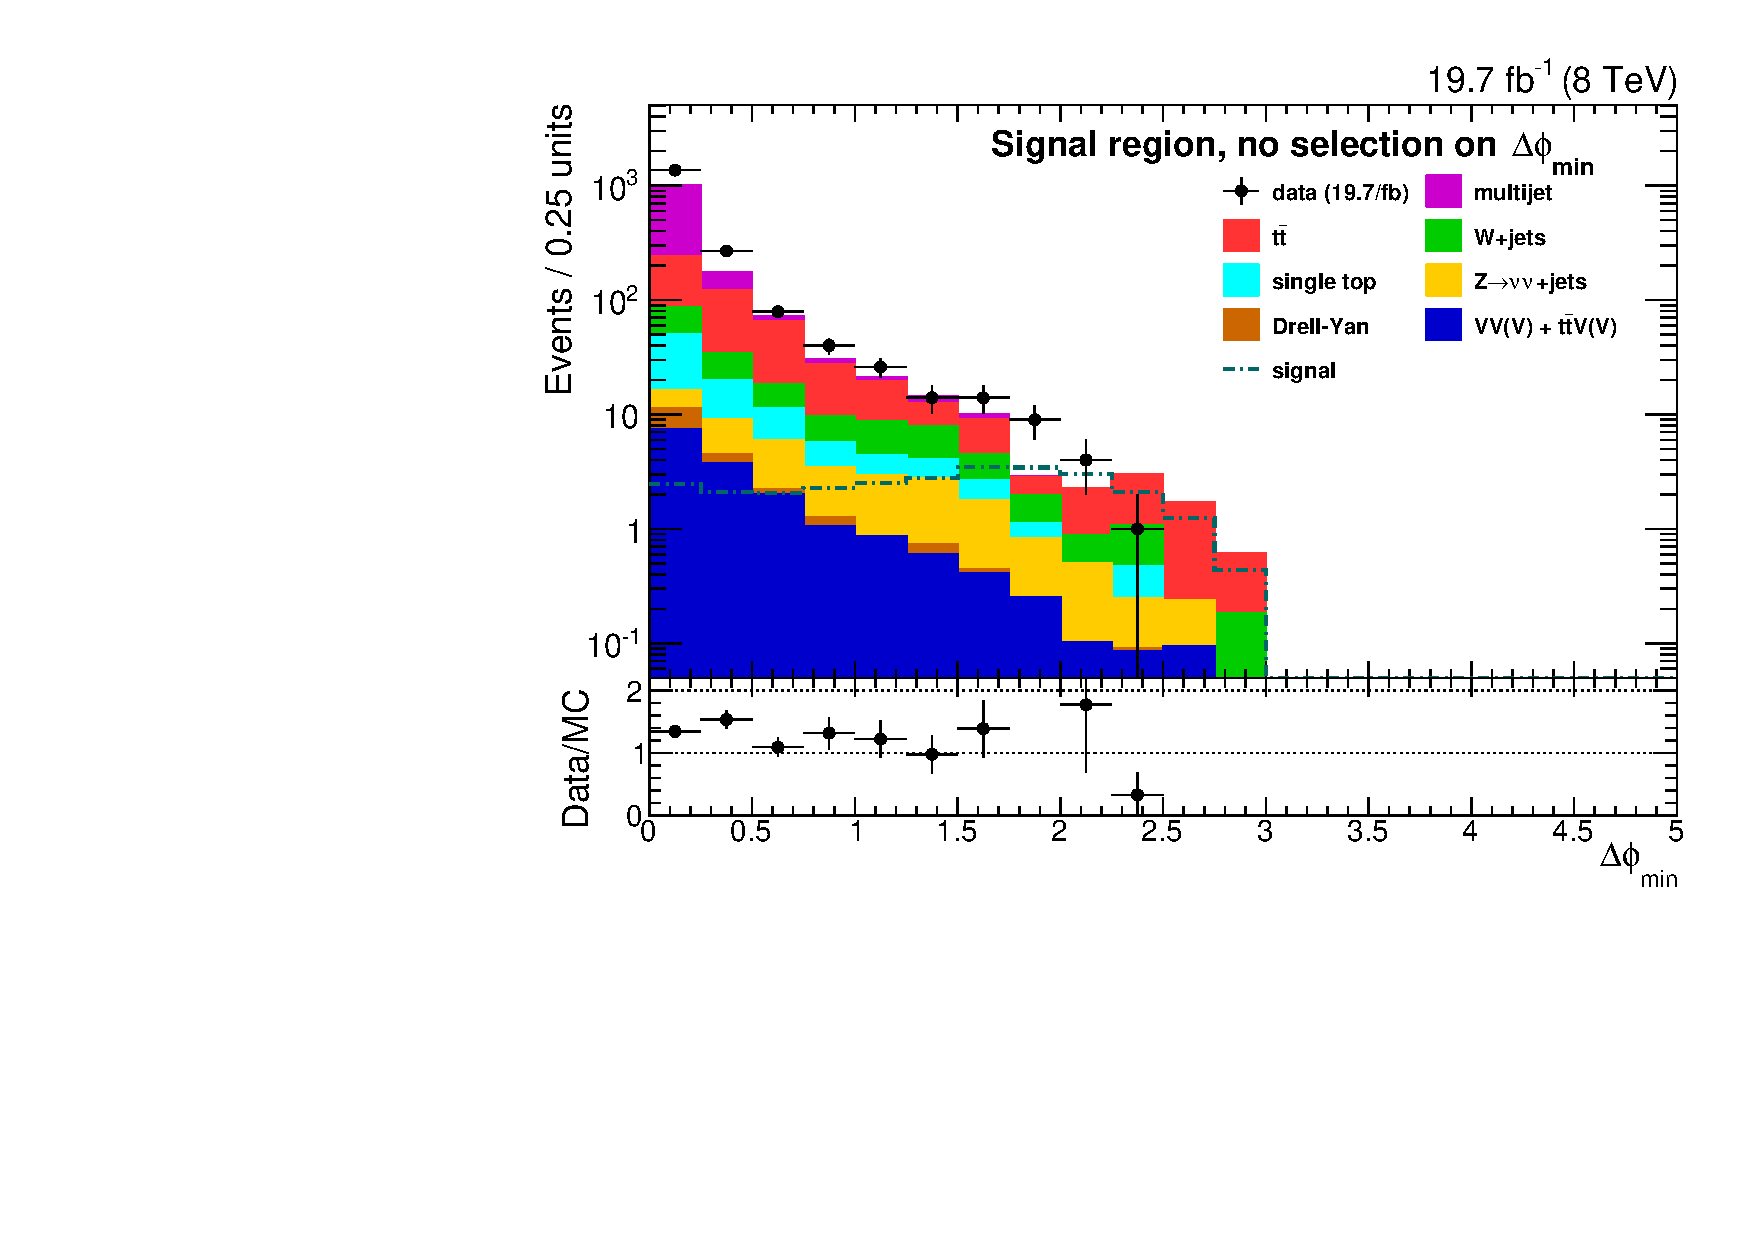
\includegraphics[width=0.49\textwidth]{figures/DataMC/DataMC_minDeltaPhi_g1Mbg1W0Ll_rebin}
% \caption{Data/MC comparison plot for the full $\Delta\phi_{min}$ distribution with all signal region
% requirements applied except $\Delta\phi_{min} > 0.5$.
% \label{fig:DataMC_SignalRegion_mdphi}}
% \end{figure}
% 
% \begin{figure}[htbp]
%  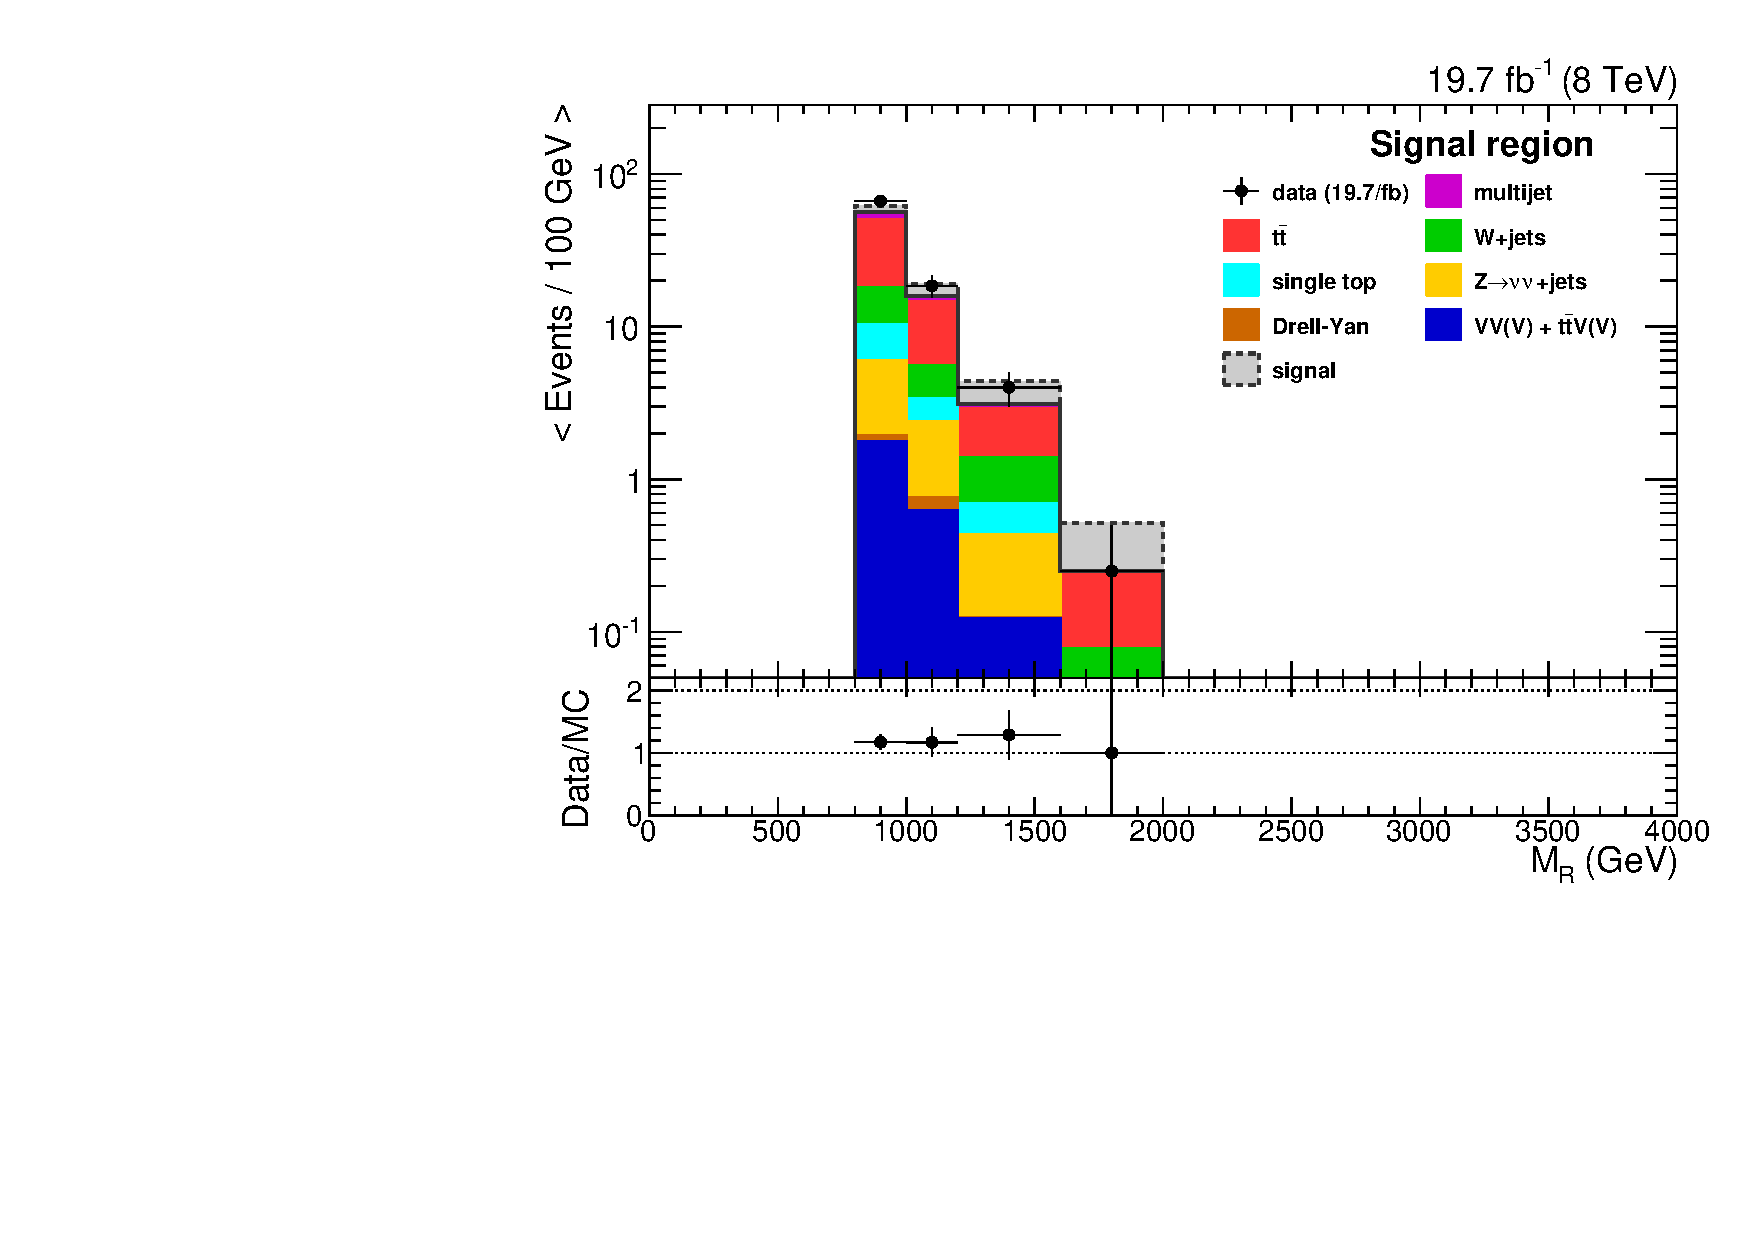
\includegraphics[width=0.49\textwidth]{figures/DataMC/DataMC_MR_g1Mbg1W0Ll_mdPhig0p5_width}
%  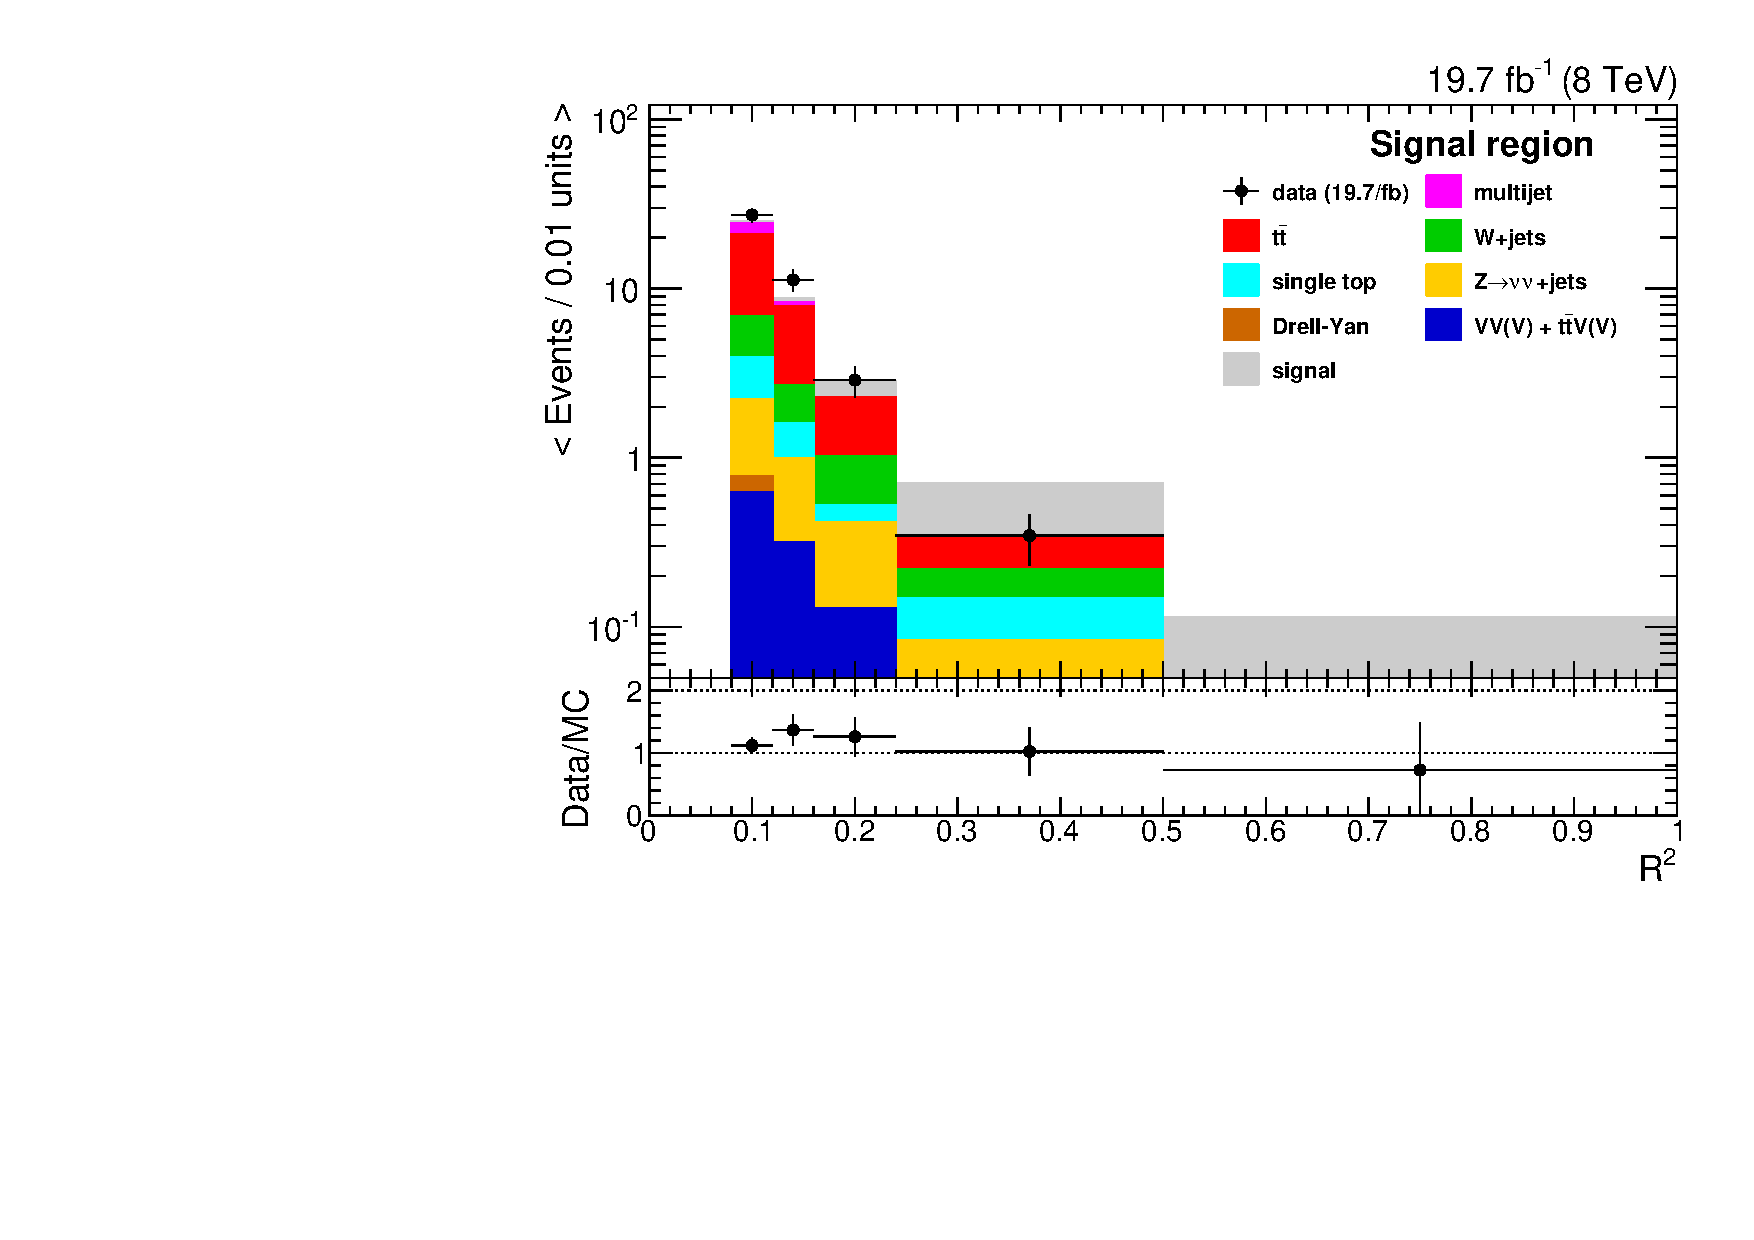
\includegraphics[width=0.49\textwidth]{figures/DataMC/DataMC_R2_g1Mbg1W0Ll_mdPhig0p5_width}
% \caption{For illustration only: Data/MC comparison plot of $M_R$ (left) and $R^2$ (right) in the
% signal region requiring $\Delta\phi_{min} > 0.5$.
% \label{fig:DataMC_SignalRegion_MR_R2_mdphig0p5}}
% \end{figure}
% 
% 
% \begin{figure}[p]
%  \includegraphics[width=0.49\textwidth]{figures/DataMC/DataMC_njets_g1Mbg1W0Ll_mdPhig0p5}
%  \includegraphics[width=0.49\textwidth]{figures/DataMC/DataMC_nbjets_g1Mbg1W0Ll_mdPhig0p5}
% 
%  \includegraphics[width=0.49\textwidth]{figures/DataMC/DataMC_met_g1Mbg1W0Ll_mdPhig0p5}
%  \includegraphics[width=0.49\textwidth]{figures/DataMC/DataMC_jet1pt_g1Mbg1W0Ll_mdPhig0p5}
% 
%  \includegraphics[width=0.49\textwidth]{figures/DataMC/DataMC_jet2pt_g1Mbg1W0Ll_mdPhig0p5}
%  \includegraphics[width=0.49\textwidth]{figures/DataMC/DataMC_jet3pt_g1Mbg1W0Ll_mdPhig0p5}
% \caption{For illustration only: Data/MC comparison plot of various event quantities in the signal
% region requiring $\Delta\phi_{min} > 0.5$: 
% [top] jet multiplicity (left) and b-tagged jet multiplicity (right);
% [middle] missing transverse energy (left) and \pt of the highest \pt jet (right);
% [bottom] \pt of the second (left) and third (right) highest \pt jet. 
% \label{fig:DataMC_SignalRegion_mdphig0p5}}
% \end{figure}
% 
% \begin{figure}[htbp]
%  \includegraphics[width=0.49\textwidth]{figures/DataMC/DataMC_Wpt_g1Mbg1W0Ll_mdPhig0p5}
%  \includegraphics[width=0.49\textwidth]{figures/Shapes/comparison_Wpt}
% \caption{For illustration only: [left] Data/MC comparison plot of $\pt(W)$ in the signal region
% requiring $\Delta\phi_{min} > 0.5$.
% [right] Comparison of the $\pt(W)$ distribution for signal and total background. Both distributions
% are normalized to unit area.
% \label{fig:Wpt_SignalRegion}}
% \end{figure}
% 
% To get a sense of the signal sensitivity we can expect, we show the signal efficiencies, expected
% number of events and significances $\frac{S}{\sqrt{B}}$ for the T1ttcc simplified model in
% figure~\ref{fig:eff_T1ttcc}, for the T1t1t model in figure~\ref{fig:eff_T1t1t} and for the T2tt
% model in figure~\ref{fig:eff_T2tt}. 
% Efficiencies of up to 7\% in the most boosted regimes of these scans are reached. 
% For the T1ttcc model a drop in efficiency is observed for the strip with lowest neutralino mass
% ($m_{\chi_1^0} = 1\GeV$). 
% For strips with higher LSP masses, the LSP will end up with higher momentum than the charm. For the
% lowest LSP mass however, the LSP and the charm have about equal mass, so after the boost they will
% receive about equal amounts of momentum. This results in a lower \ETm spectrum, and in the end a
% lower efficiency. 
% This is explained in more detail in Appendix~\ref{app:eff_drop}. 
% 
% \begin{figure}[htbp]
%  \centering
%  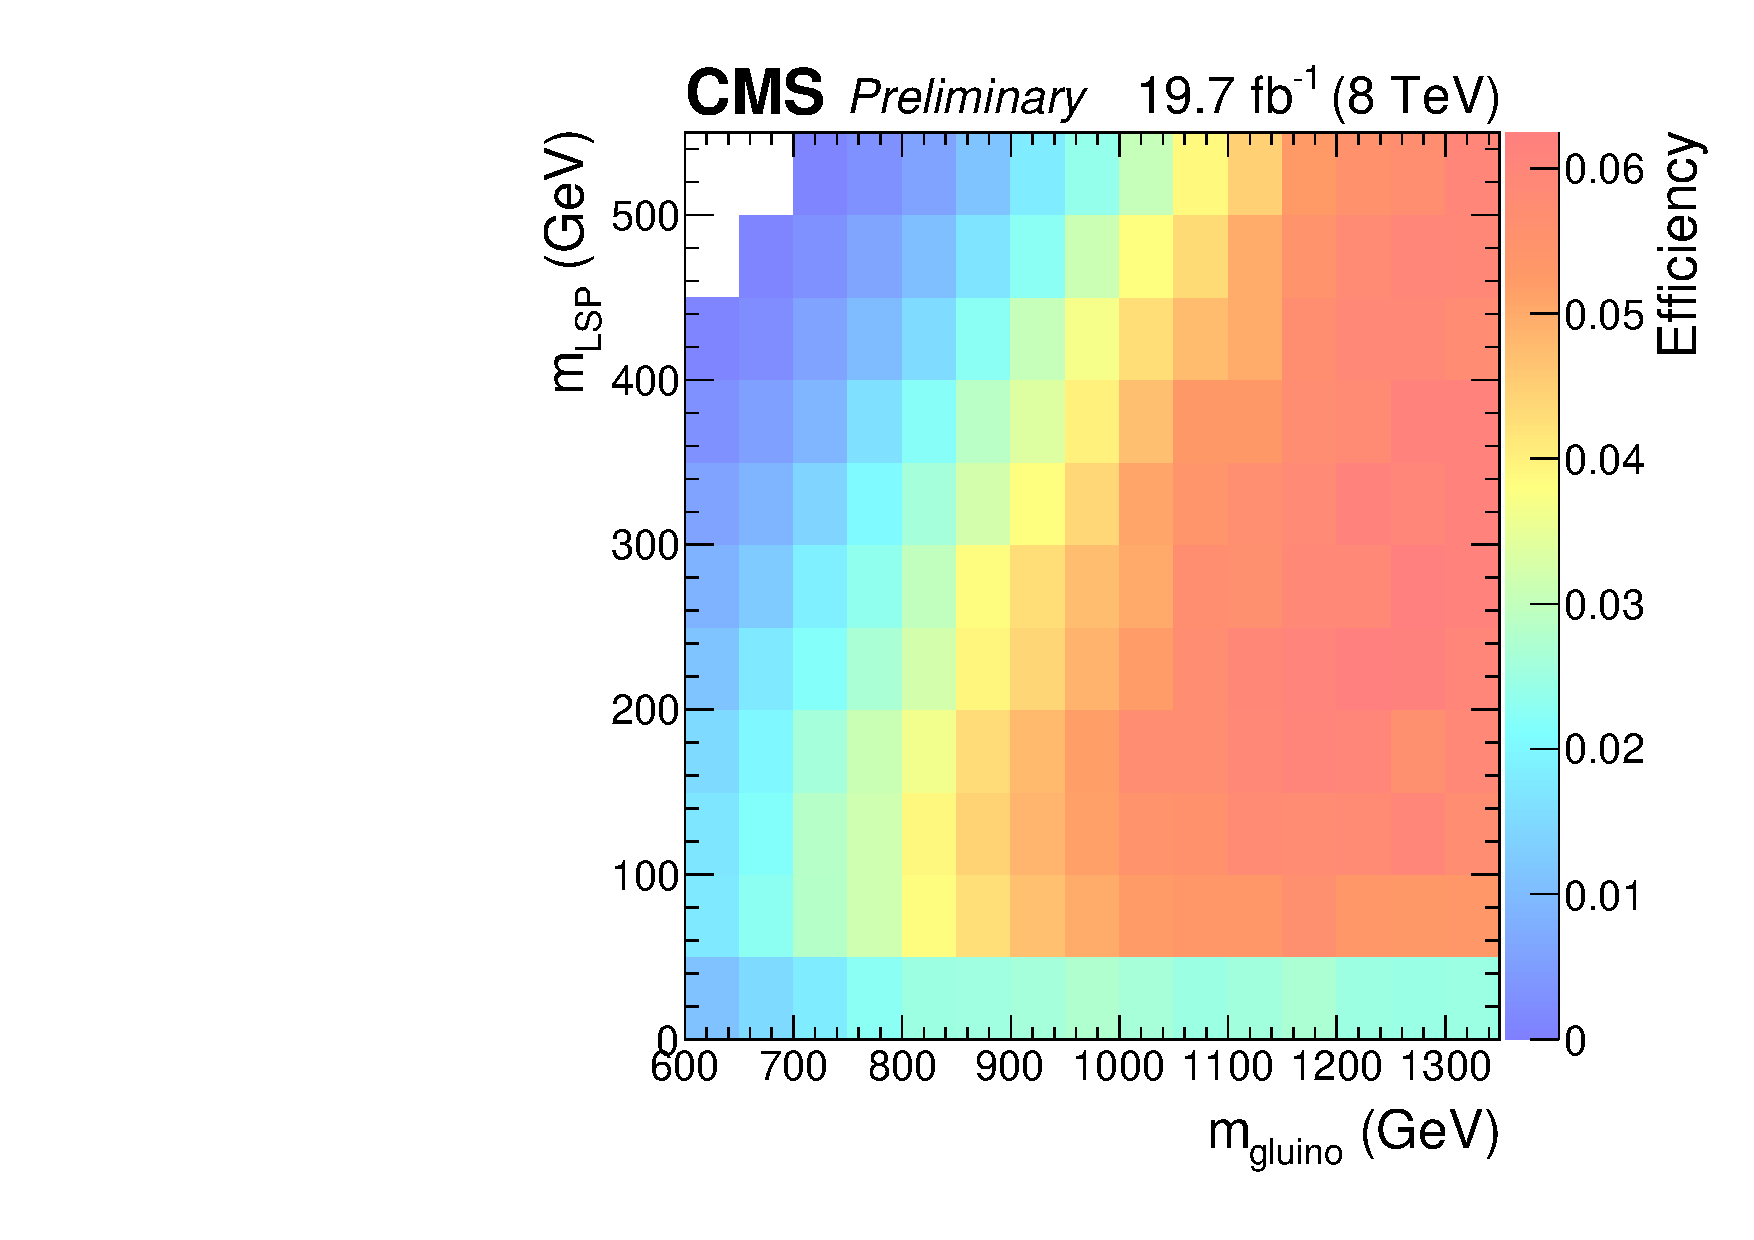
\includegraphics[width=0.3\textwidth]{figures/T1ttcc/efficiency_T1ttcc_DM-10_g1Mbg1W0Ll_mdPhig0p5}
% ~
%  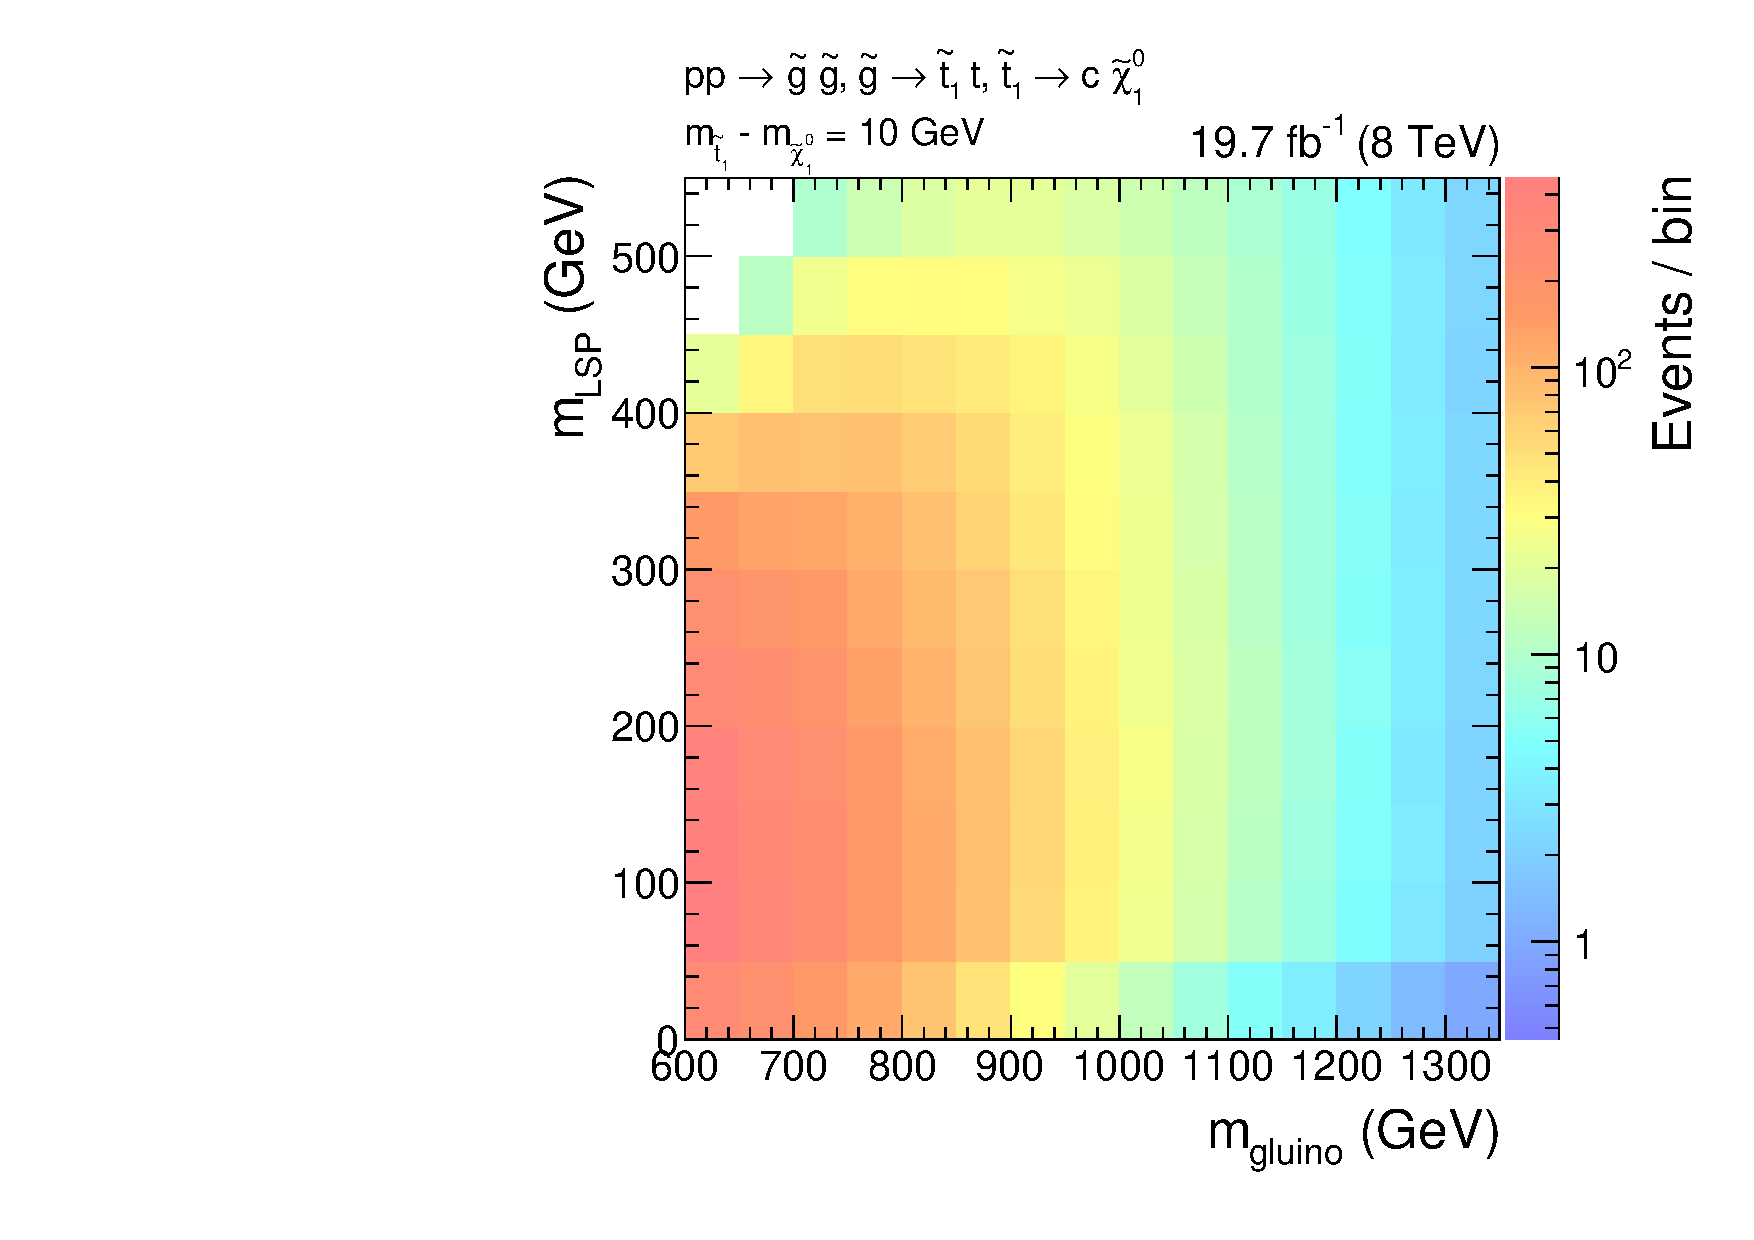
\includegraphics[width=0.3\textwidth]{figures/T1ttcc/events_T1ttcc_DM-10_g1Mbg1W0Ll_mdPhig0p5} ~
%  \includegraphics[width=0.3\textwidth]{figures/T1ttcc/significance_T1ttcc_DM-10_g1Mbg1W0Ll_mdPhig0p5
% }
% 
%  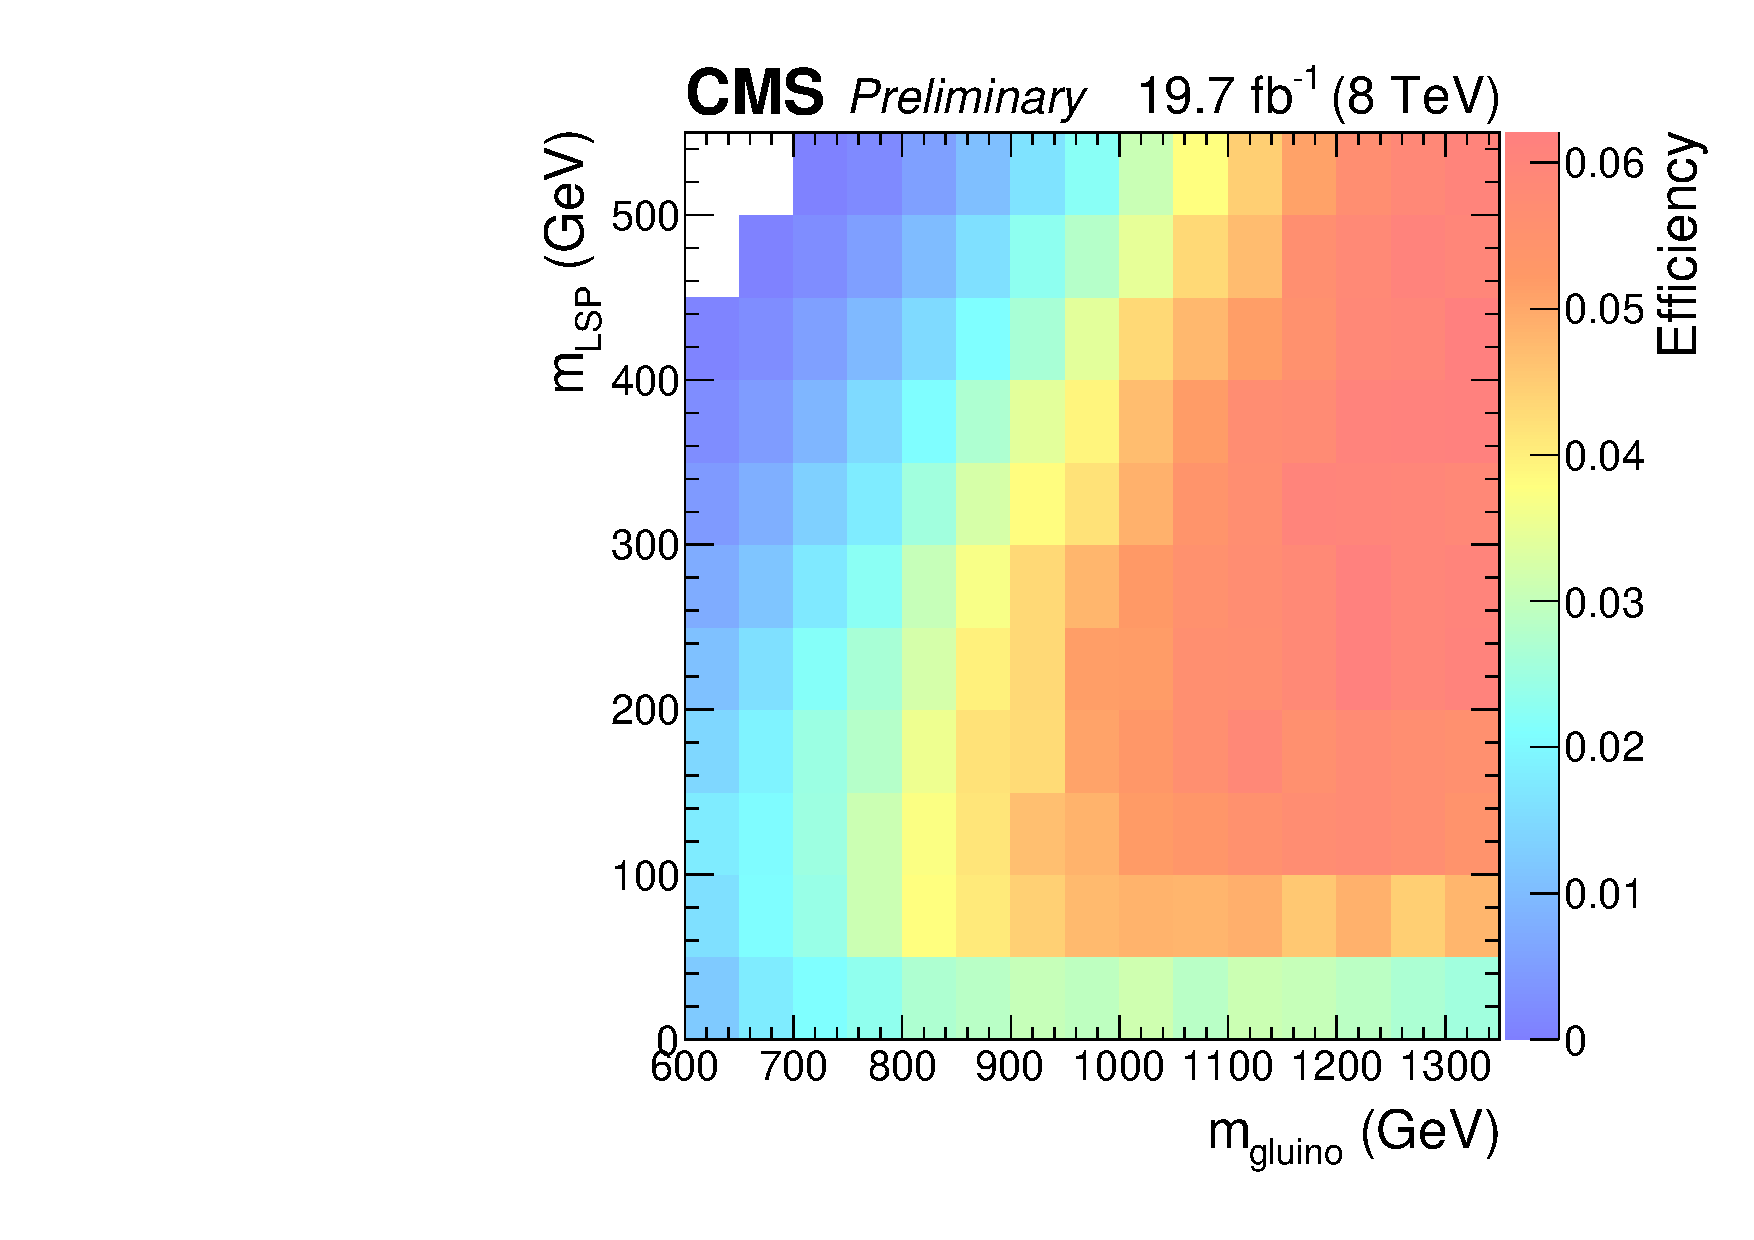
\includegraphics[width=0.3\textwidth]{figures/T1ttcc/efficiency_T1ttcc_DM-25_g1Mbg1W0Ll_mdPhig0p5}
% ~
%  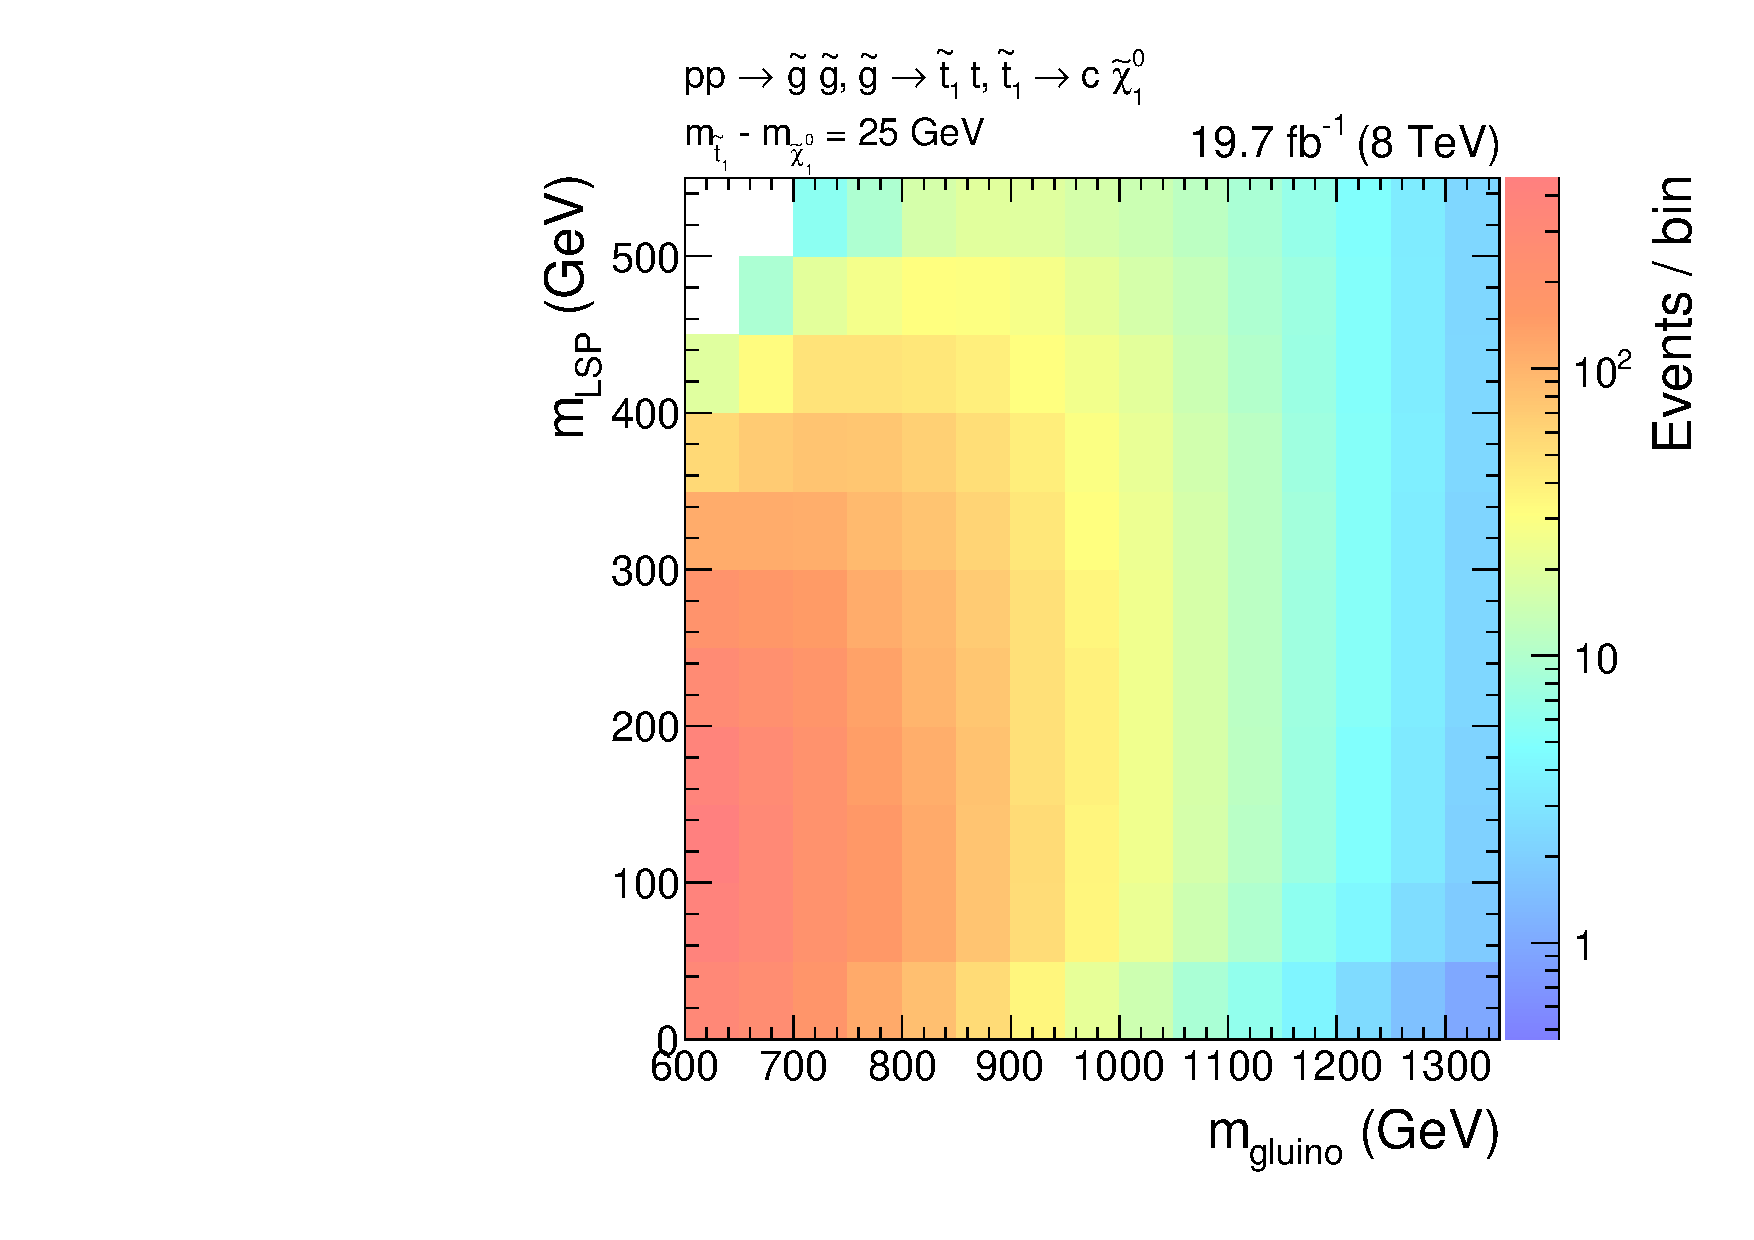
\includegraphics[width=0.3\textwidth]{figures/T1ttcc/events_T1ttcc_DM-25_g1Mbg1W0Ll_mdPhig0p5} ~
%  \includegraphics[width=0.3\textwidth]{figures/T1ttcc/significance_T1ttcc_DM-25_g1Mbg1W0Ll_mdPhig0p5
% }
% 
%  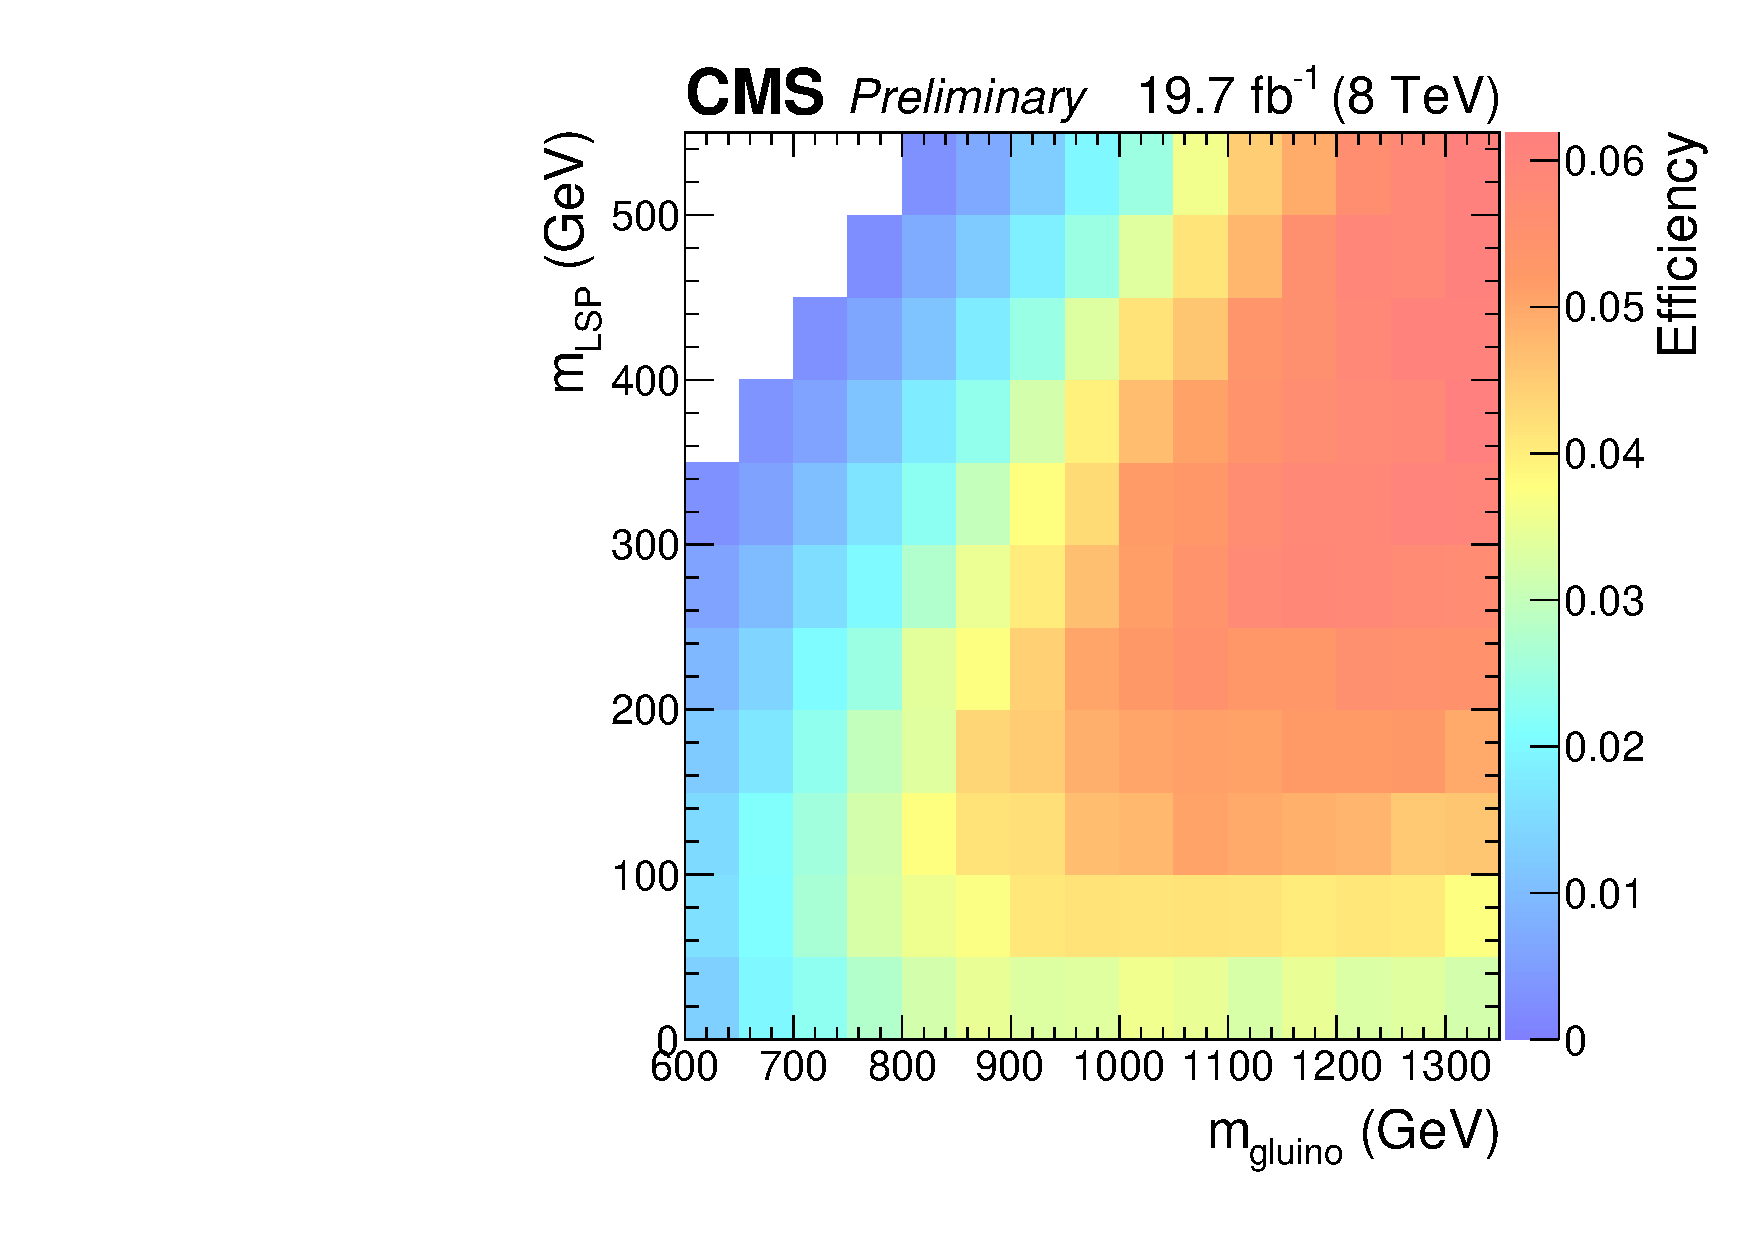
\includegraphics[width=0.3\textwidth]{figures/T1ttcc/efficiency_T1ttcc_DM-80_g1Mbg1W0Ll_mdPhig0p5}
% ~
%  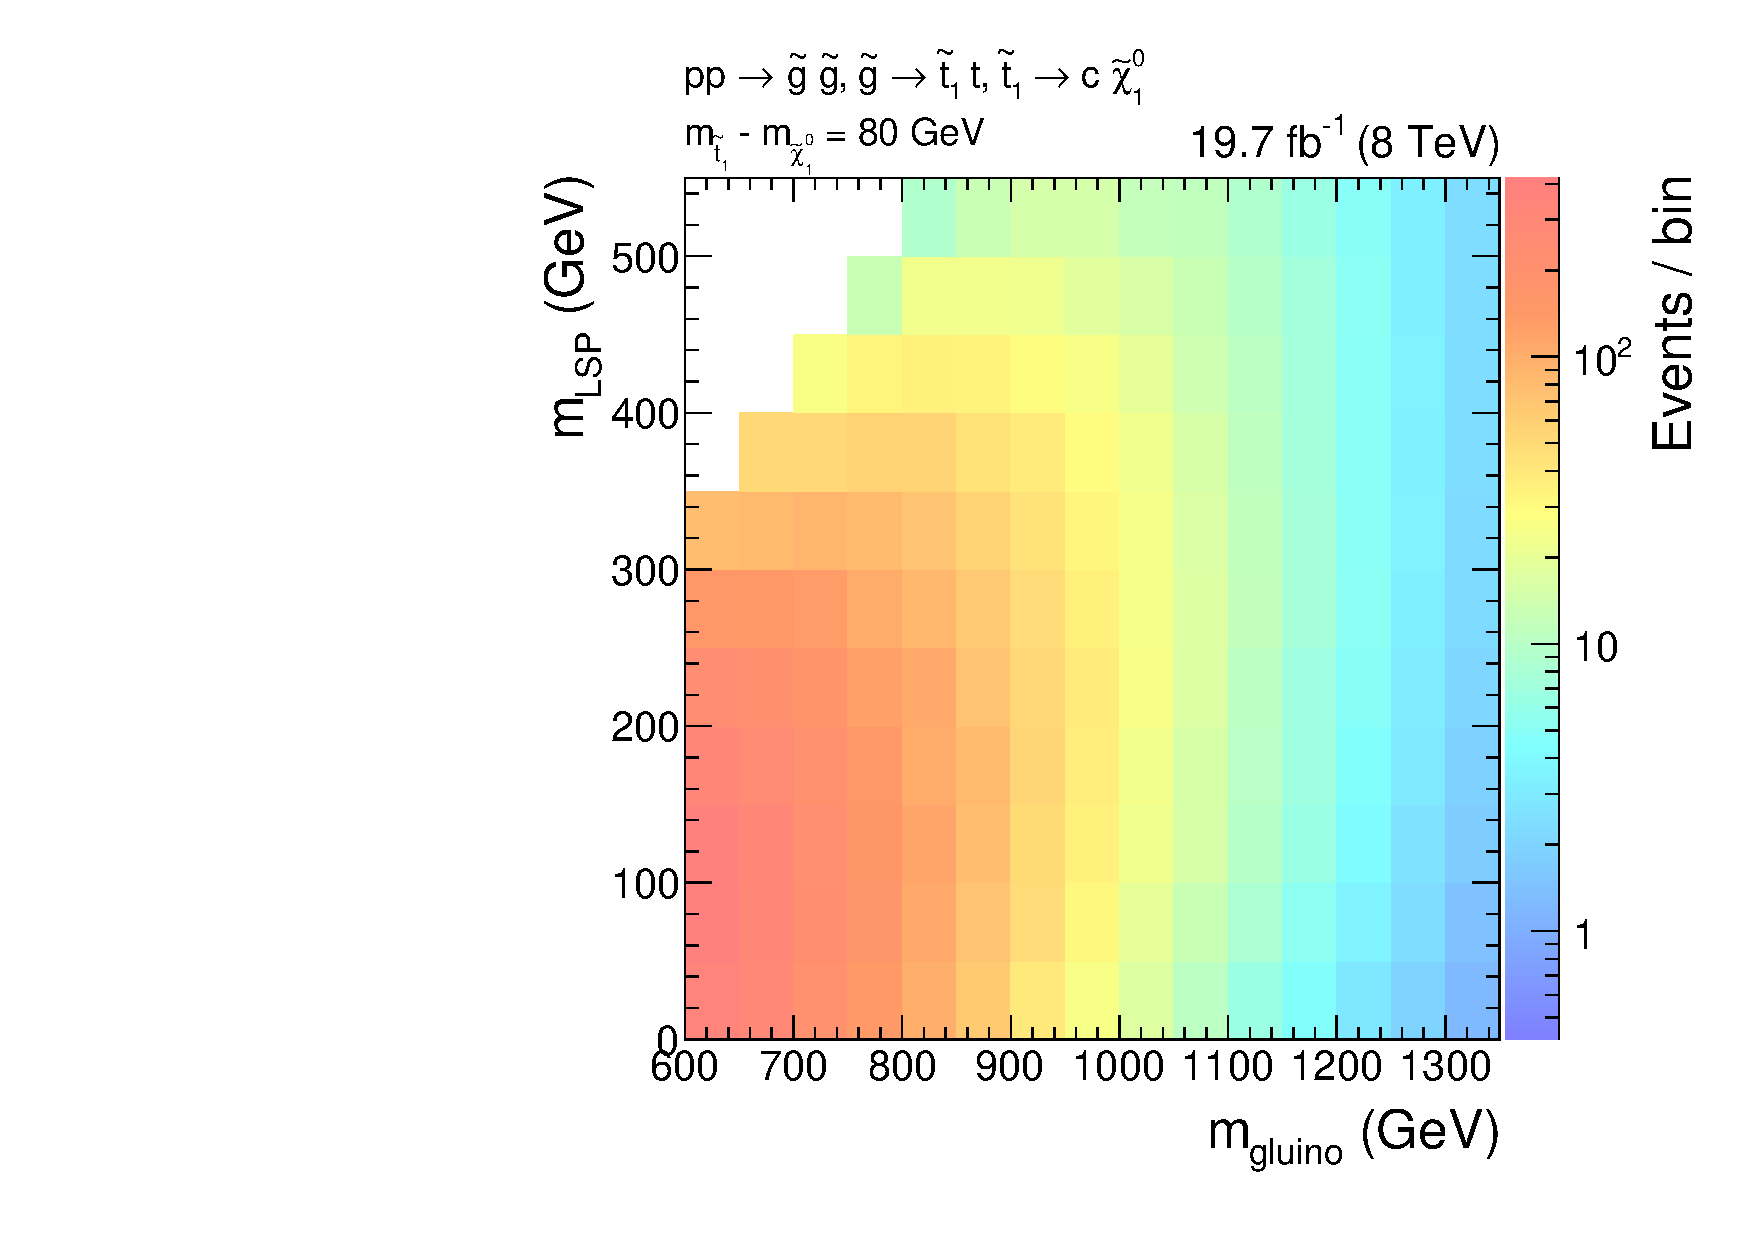
\includegraphics[width=0.3\textwidth]{figures/T1ttcc/events_T1ttcc_DM-80_g1Mbg1W0Ll_mdPhig0p5} ~
%  \includegraphics[width=0.3\textwidth]{figures/T1ttcc/significance_T1ttcc_DM-80_g1Mbg1W0Ll_mdPhig0p5
% }
%  \caption{Signal region efficiency, number of events in $19.712\textrm{fb}^{-1}$ and significance
% $\frac{S}{\sqrt{B}}$ for the T1ttcc simplified model. Three mass splittings between stop and LSP are
% considered: 10, 25 and 80 \GeV, shown in the top, middle and bottom row, respectively.
%  \label{fig:eff_T1ttcc}}
% \end{figure}
% 
% \begin{figure}[htbp]
%  \centering
%   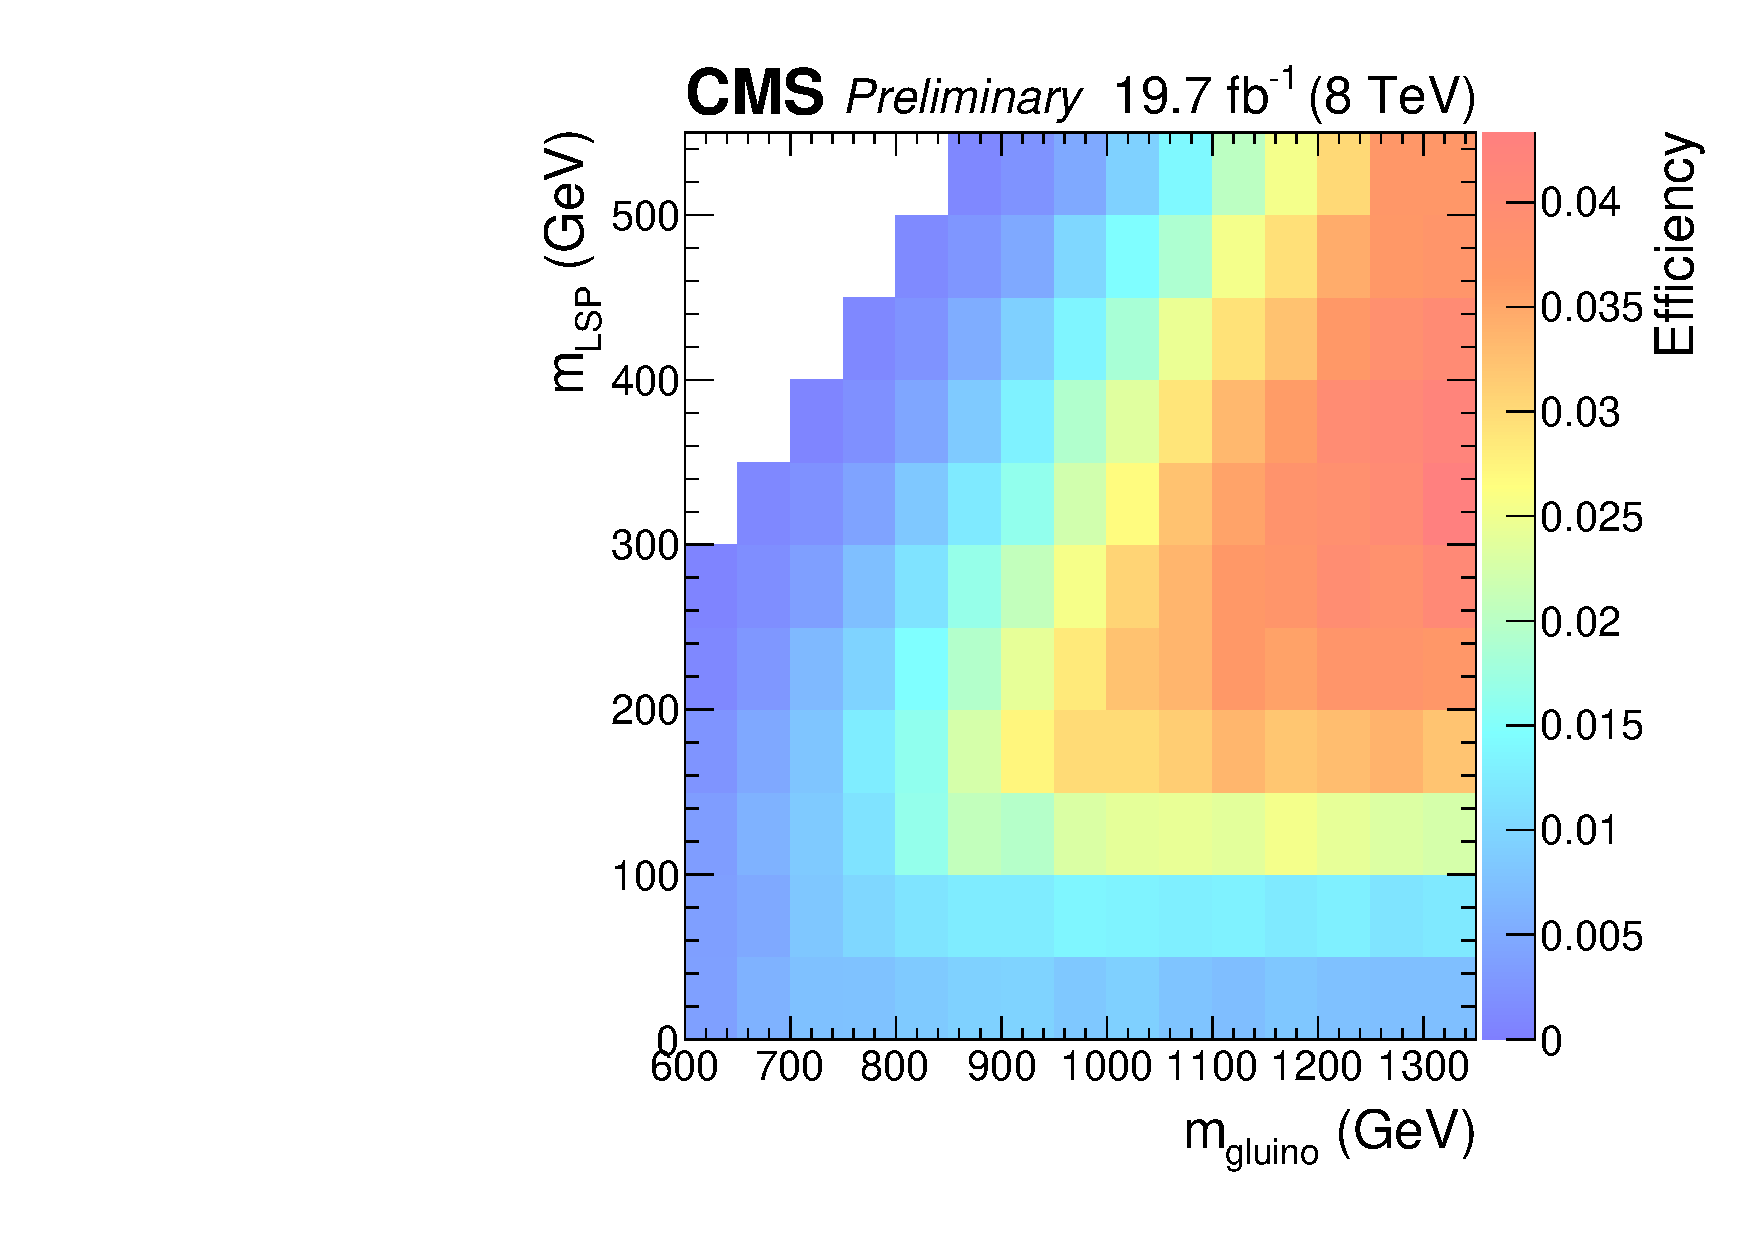
\includegraphics[width=0.3\textwidth]{figures/T1t1t/efficiency_T1t1t_g1Mbg1W0Ll_mdPhig0p5} ~
%  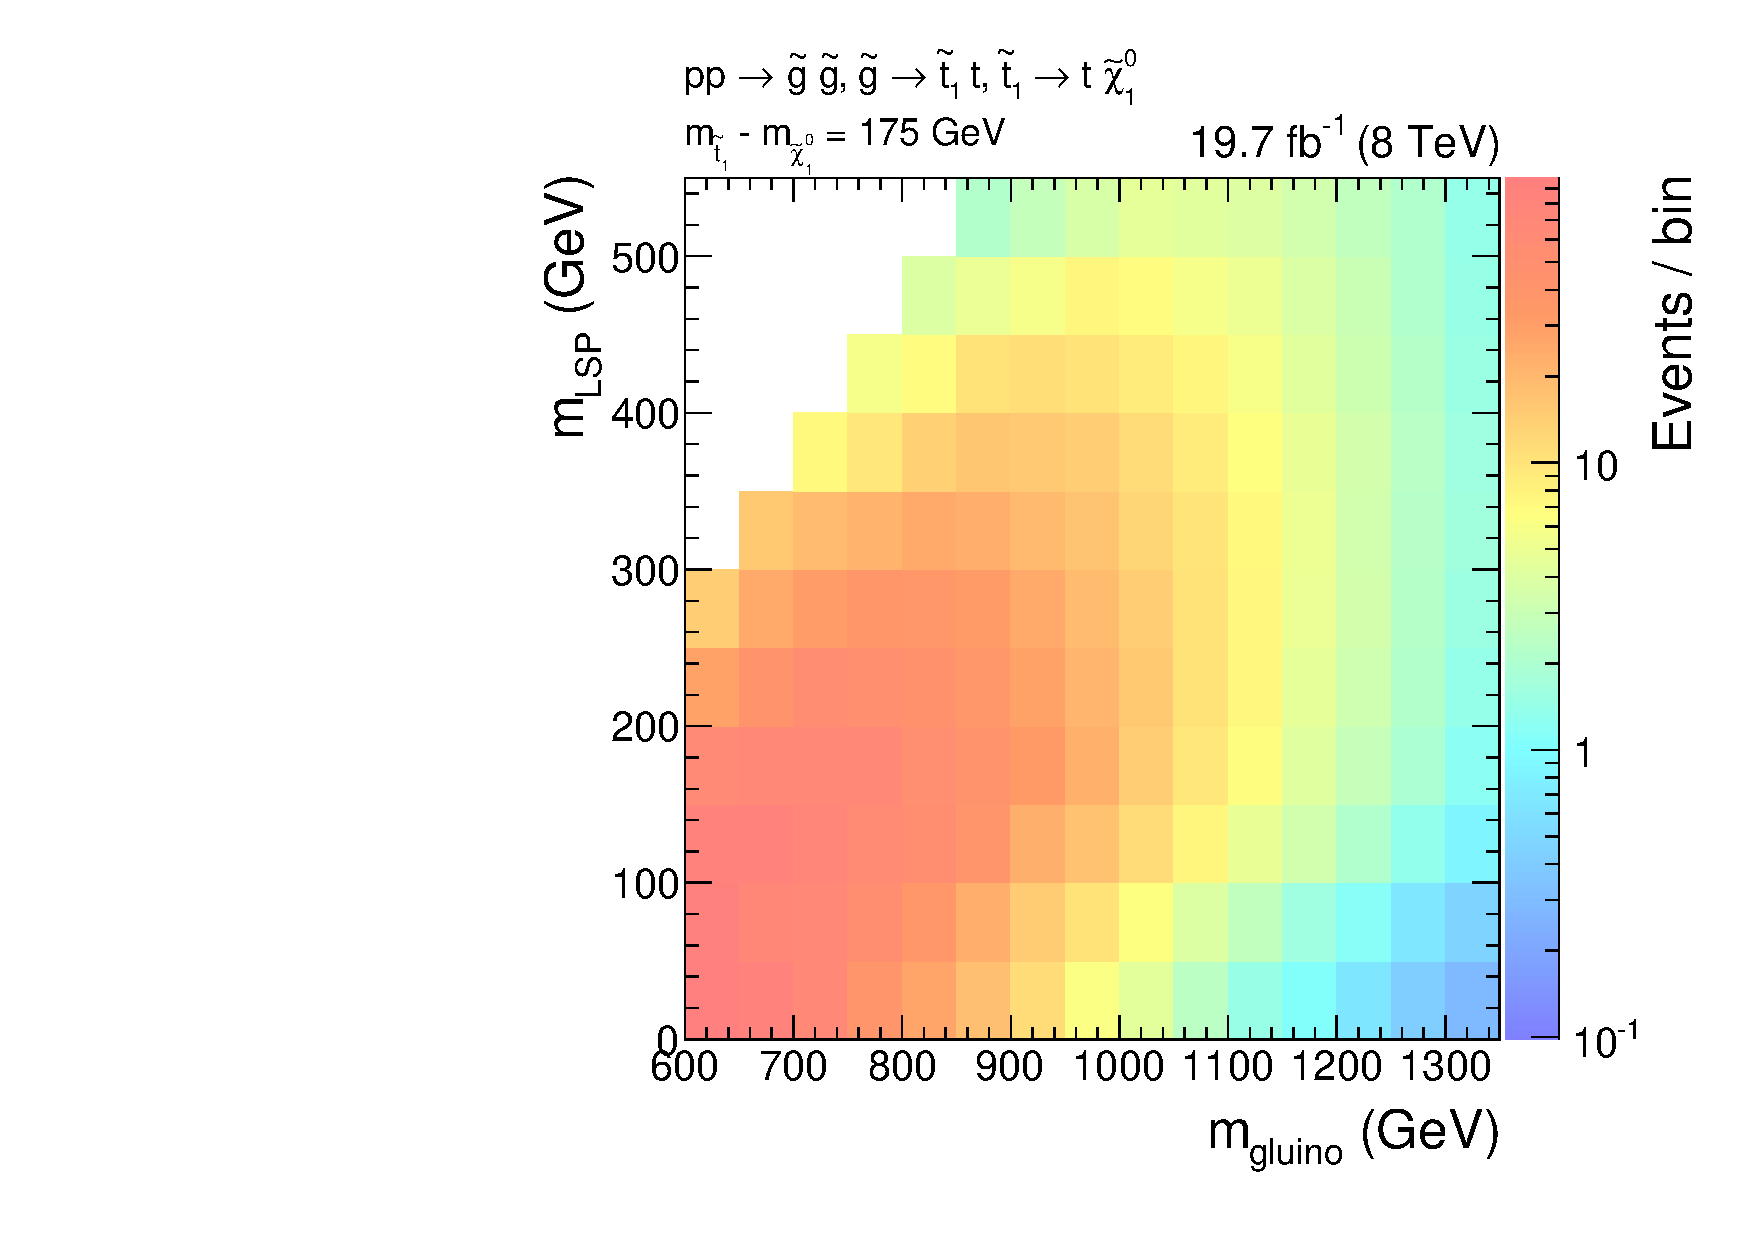
\includegraphics[width=0.3\textwidth]{figures/T1t1t/events_T1t1t_g1Mbg1W0Ll_mdPhig0p5} ~
%  \includegraphics[width=0.3\textwidth]{figures/T1t1t/significance_T1t1t_g1Mbg1W0Ll_mdPhig0p5}
%  \caption{Signal region efficiency, number of events in $19.712\textrm{fb}^{-1}$ and significance
% $\frac{S}{\sqrt{B}}$ for the T1t1t simplified model.
%  \label{fig:eff_T1t1t}}
% \end{figure}
% 
% \begin{figure}[htbp]
%  \centering
%   \includegraphics[width=0.3\textwidth]{figures/T2tt/efficiency_T2tt_g1Mbg1W0Ll_mdPhig0p5} ~
%  \includegraphics[width=0.3\textwidth]{figures/T2tt/events_T2tt_g1Mbg1W0Ll_mdPhig0p5} ~
%  \includegraphics[width=0.3\textwidth]{figures/T2tt/significance_T2tt_g1Mbg1W0Ll_mdPhig0p5}
%  \caption{Signal region efficiency, number of events in $19.712\textrm{fb}^{-1}$ and significance
% $\frac{S}{\sqrt{B}}$ for the T2tt simplified model.
%  \label{fig:eff_T2tt}}
% \end{figure}
